
\section{Ergebnisse und Interpretation}

Es gibt zwei Möglichkeiten, wie dieser Abschnitt aufgebaut sein kann. Entweder man gibt einen Teil der Ergebnisse an, diskutiert und interpretiert ihn, fährt mit dem nächsten Teil der Ergebnisse fort und so weiter. Oder man gibt alle Ergebnisse an und diskutiert sie anschließend. Die Struktur hängt von den Daten ab, die gemessen wurden. Handelt es sich um eine große Messung mit zusammenhängenden Ergebnissen, ist es oft besser, die zweite Struktur zu wählen. Handelt es sich um mehrere Einzelmessungen, ist die erste Struktur sinnvoller.\\
\\
In diesem Labor wird nur Ergebnis Datensatz erzielt, so dass die zweite Struktur sinnvoll ist. Normalerweise wird in den Laboranweisungen nach bestimmten Ergebnissen gefragt. In diesem Fall wurde ein Bode-Diagramm des Tiefpassfilters verlangt, daher sollte zumindest ein komplettes Bode-Diagramm gezeigt werden! Dies sollte ein Diagramm gemäß den MCI-Richtlinien sein, ein Beispiel ist in Abbildung \ref{fig:BodePlot} dargestellt. Falls sinnvoll (n <= 10), können die Rohdaten der Messungen in einer Tabelle dargestellt werden. 


\begin{figure}[H]
	\centering	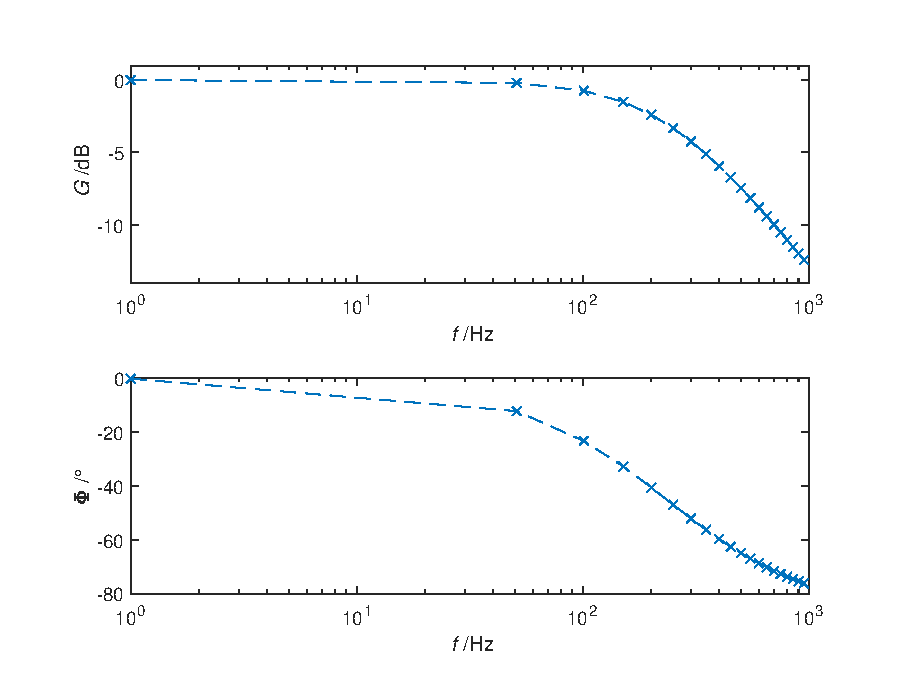
\includegraphics[width=0.9\textwidth]{images/BodePlot.eps} % eps is a nice vector graphics format exported by matlab to be used with latex.
	\caption[Gemessener Bode-Diagramm]{Das gezeigte Bode-Diagramm ist für $R$ = 68 \si{\kilo \ohm} und $C$ = 10 \si{\nano \farad} gültig. Bei Messungen ist es wichtig, die Datenpunkte zu markieren und nicht eine durchgezogene Linie zu verwenden. Diagramme sollten keine Titel tragen, und die Achsen müssen mit Symbol und Einheit beschriftet werden. Gibt es mehr als eine Linie in einem Diagramm, verwenden Sie verschiedene Markierungen und/oder Linienstile sowie eine Legende. In diesem Fall handelt es sich um 20 Datenpunkte. Da die Verstärkung $G$ und die Phase $\Phi$ aus den gemessenen Spannungen berechnet werden müssen, sollte die Gleichung ebenfalls angegeben werden.} 
	\label{fig:BodePlot}
\end{figure}


Nachdem die Ergebnisse festgestellt wurden, sollten sie diskutiert und interpretiert werden. Was können Sie sehen, und was bedeutet das? Stimmen die Ergebnisse mit Ihren Erwartungen überein? Was sind mögliche Messunsicherheiten? War die Messung erfolgreich? Wie nahe lag z.B. die gemessene Grenzfrequenz an der theoretischen, und warum weichen sie möglicherweise ab?


% After this chapter there will only be the lists and literature.